%Preamble

\documentclass[10pt,a4paper,oneside]{report}
%\usepackage{amsmath,amsthm,amssymb}
\usepackage{multirow}
\usepackage[table,xcdraw]{xcolor}
\usepackage{array}
\usepackage{colortbl}
%\usepackage{lipsum}
\usepackage{graphicx}

\pagestyle{empty}

%\title{Activities and Schedule}
\begin{document}%opening statement-body
%\maketitle
\setlength{\parindent}{0pt} %

\vspace{-4cm}\section{Activities and Schedule}

\textbf{Description of Activity Allocation:}
Our project has 13 main activities, five of which are done jointly by all team members and the other seven are allocated to the most suitable team members based on their strengths. For example, Kin is good at research and has flexible working hours, so she was selected as the leader of our team, responsible for making Literature Review, deciding research questions and presentation slides. The following table shows the strengths of the group members and the activities they are responsible for.
\begin{table}[htbp]
	\resizebox{1\textwidth}{!}{
	\begin{tabular}{|1|cll|}
		\hline
		\multicolumn{1}{|c|}{Tasks} & \multicolumn{1}{c|}{\cellcolor[HTML]{FFFFFF}Members Name} & \multicolumn{1}{c|}{Members Roles} & \multicolumn{1}{c|}{Members Strengths and Experiences} \\ \hline
		Decide roles of members & \multicolumn{3}{c|}{All Members} \\ \hline
		Decide research question & \multicolumn{3}{c|}{All Members} \\ \hline
		Write project plan & \multicolumn{3}{c|}{All Members} \\ \hline
		Write report & \multicolumn{3}{c|}{All Members} \\ \hline
		Source external data & \multicolumn{3}{c|}{All Members} \\ \hline
		Record presentation & \multicolumn{3}{c|}{All Members} \\ \hline
		& \multicolumn{1}{c|}{Kin Cheang} & \multicolumn{1}{c|}{Team Leader} & Coding, Research, Mathematics \\ \cline{2-4} 
		\multirow{-2}{*}{Literature review} & \multicolumn{1}{c|}{Zining Wang} & \multicolumn{1}{c|}{Data Analyst} & Coding, Data visualization, Research \\ \hline
		& \multicolumn{1}{c|}{Alexander Hodges} & \multicolumn{1}{c|}{} & Coding, Machine learning, Mathematics \\ \cline{2-2} \cline{4-4} 
		\multirow{-2}{*}{Research methods and software} & \multicolumn{1}{c|}{Zining Wang} & \multicolumn{1}{c|}{\multirow{-2}{*}{Data Analyst}} & Coding, Data visualization, Research \\ \hline
		& \multicolumn{1}{c|}{Kourosh Shaban} & \multicolumn{1}{c|}{} & Coding, Machine learning, Mathematics \\ \cline{2-2} \cline{4-4} 
		& \multicolumn{1}{c|}{Alexander Hodges} & \multicolumn{1}{c|}{} & Coding, Machine learning, Mathematics \\ \cline{2-2} \cline{4-4} 
		\multirow{-3}{*}{Data preparation} & \multicolumn{1}{c|}{Zining Wang} & \multicolumn{1}{c|}{\multirow{-3}{*}{Data Analyst}} & Coding, Data visualization, Research \\ \hline
		& \multicolumn{1}{l|}{Kourosh Shaban} & \multicolumn{1}{l|}{} & Coding, Machine learning, Mathematics \\ \cline{2-2} \cline{4-4} 
		& \multicolumn{1}{l|}{Alexander Hodges} & \multicolumn{1}{l|}{} & Coding, Machine learning, Mathematics \\ \cline{2-2} \cline{4-4} 
		\multirow{-3}{*}{Data analysis} & \multicolumn{1}{l|}{Zining Wang} & \multicolumn{1}{l|}{\multirow{-3}{*}{Data Analyst}} & Coding, Data visualization, Research \\ \hline
		& \multicolumn{1}{l|}{Kourosh Shaban} & \multicolumn{1}{l|}{} & Coding, Machine learning, Mathematics \\ \cline{2-2} \cline{4-4} 
		& \multicolumn{1}{l|}{Alexander Hodges} & \multicolumn{1}{l|}{} & Coding, Machine learning, Mathematics \\ \cline{2-2} \cline{4-4} 
		\multirow{-3}{*}{Modelling} & \multicolumn{1}{l|}{Zining Wang} & \multicolumn{1}{l|}{\multirow{-3}{*}{Data Analyst}} & Coding, Data visualization, Research \\ \hline
		& \multicolumn{1}{l|}{Kourosh Shaban} & \multicolumn{1}{l|}{} & Coding, Machine learning, Mathematics \\ \cline{2-2} \cline{4-4} 
		& \multicolumn{1}{l|}{Alexander Hodges} & \multicolumn{1}{l|}{} & Coding, Machine learning, Mathematics \\ \cline{2-2} \cline{4-4} 
		\multirow{-3}{*}{Evaluation of model} & \multicolumn{1}{l|}{Zining Wang} & \multicolumn{1}{l|}{\multirow{-3}{*}{Data Analyst}} & Coding, Data visualization, Research \\ \hline
		Presentation slides & \multicolumn{1}{l|}{Kin Cheang} & \multicolumn{1}{l|}{Team Leader} & Coding, Research, Mathematics \\ \hline
	\end{tabular}}
\end{table}


\textbf{Setting the start and end time of each activity:}
The start time and end time of each activity are set based on the due time of each assignment in the course. To give team members enough time to review work and respond to unexpected issues, activities end one day earlier than the actual due date for each assignment. For example, the deadline for the final report is October 7, and the deadline for our group is October 6.

\textbf{Description of project plan and schedule (Figure 1):}
Project plan and schedule custom gantt charts made in excel. In order to make team members easy to use, gantt chart has only two manual functions: \item One is the name section in the upper right corner of the chart, and team members can view the progress of individual members/team members by clicking on the single/multiple name option. \item The other function is timeline cover, which allows members to drag the right side of the timeline cover to any date, with past times and completed activities in the dark side and future times and unfinished activities in the bright side.	


\newpage
	\begin{figure}[htbp]%opening statement-body
		\centering
		\vspace{-4cm}
		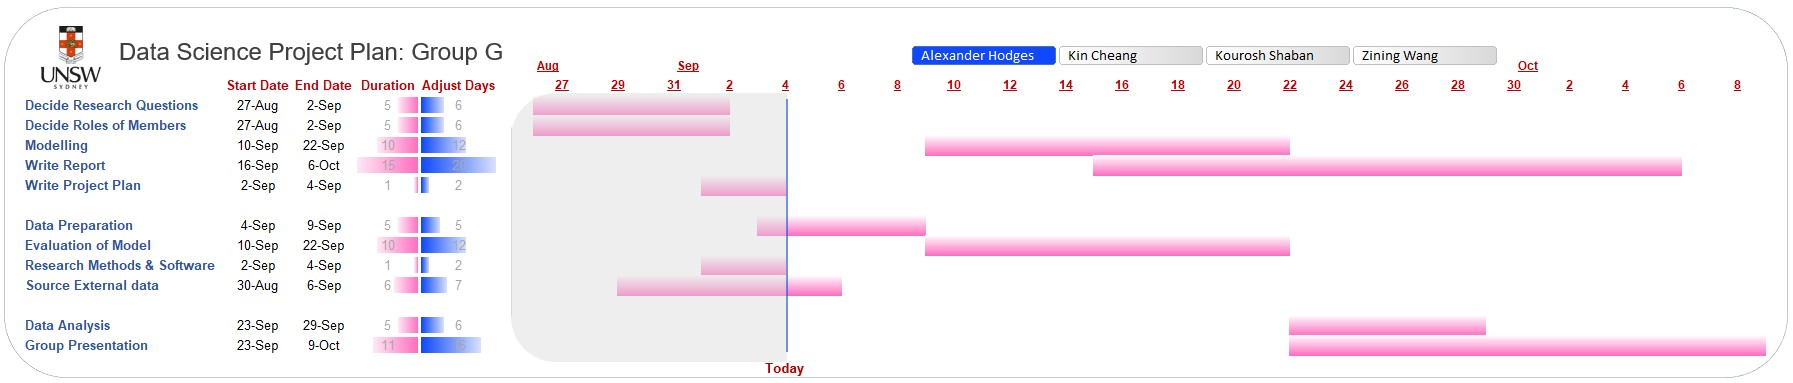
\includegraphics[scale=0.58,angle=270]{C:/Users/Josh/Desktop/GanttChart.jpg}
		\caption{Project Plan and Timeline}
		%\label{fig:Project Plan and Timeline}
	\end{figure}%closing statement-body
	
\end{document}%closing statement-body
